\section{Background}

\note{jk: Add an introductory paragraph which discuss what are you going to talk
in the background section}

\vspace{1em}
\subsection{TeraHeap}
TeraHeap is a system that eliminates S/D overhead and expensive GC scans for a
large portion of the objects in big data frameworks. TeraHeap enhances the
managed runtime environment, particularly the Java Virtual Machine (JVM). It
introduces a supplementary heap, designed for high-capacity storage, alongside
the primary heap. This secondary heap utilizes fast storage and allows direct
access to objects without the need for serialization or deserialization.
Additionally, TeraHeap minimizes the garbage collection overhead by preventing
the garbage collector from scanning the secondary heap. It takes advantage of
frameworks' capability to designate certain objects for off-heap allocation and
provides them with a hint-based method for relocating these objects to the
secondary heap. 

\subsection{Network Block Device}
 \note{jk: write the full name of NBD in the title}

 \note{jk: we first write the full name and then the accronym e.g., Network
 Block Device (NBD). Fix it everywhere...} NBD (Network Block Device) is a
 network protocol that can be used to export a block device from a server where
 the block device resides to a client. There are multiple NBD implementations
 \note{jk: which??? provide more context} we will focus on the Network Block
 Device (TCP version). \note{jk: Why you focus on TCP implementation?} 

  \begin{figure}[h]
    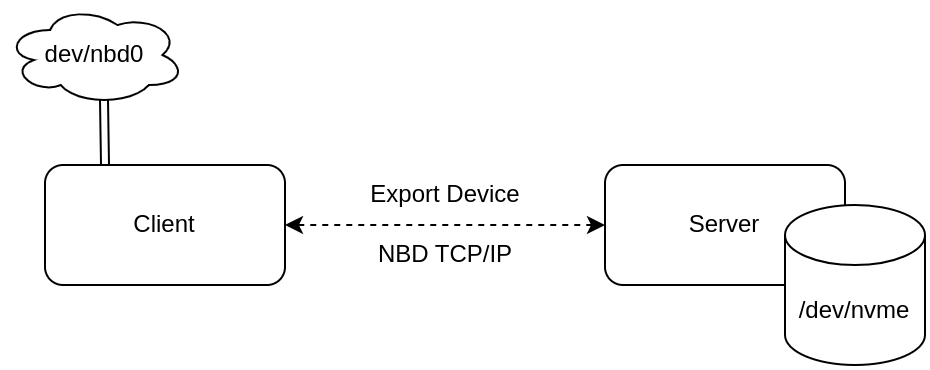
\includegraphics[scale=0.3]{figures/nbd-path.png}\\
    \caption{Overview of an NBD system.}
  \end{figure}

  \note{jk: mention which figure shows that... E.g., Figure...} With this implementation compiled in the kernel we can use 2 drivers-modules
  the nbd-client and the nbd-server. The nbd-client usually resides in the OS kernel
  and exposes a block device interface to the rest of the kernel, so that it may
  appear as an ordinary, directly-attached storage device. The client passes the
  block requests to the NBD driver where they are encapsulated as NBD network
  messages and sent to the server via TCP. Finally the User-Space server upon
  receiving the NBD request issues standard I/O to the relevant block device and
  then responds. 

  \begin{figure}[h]
    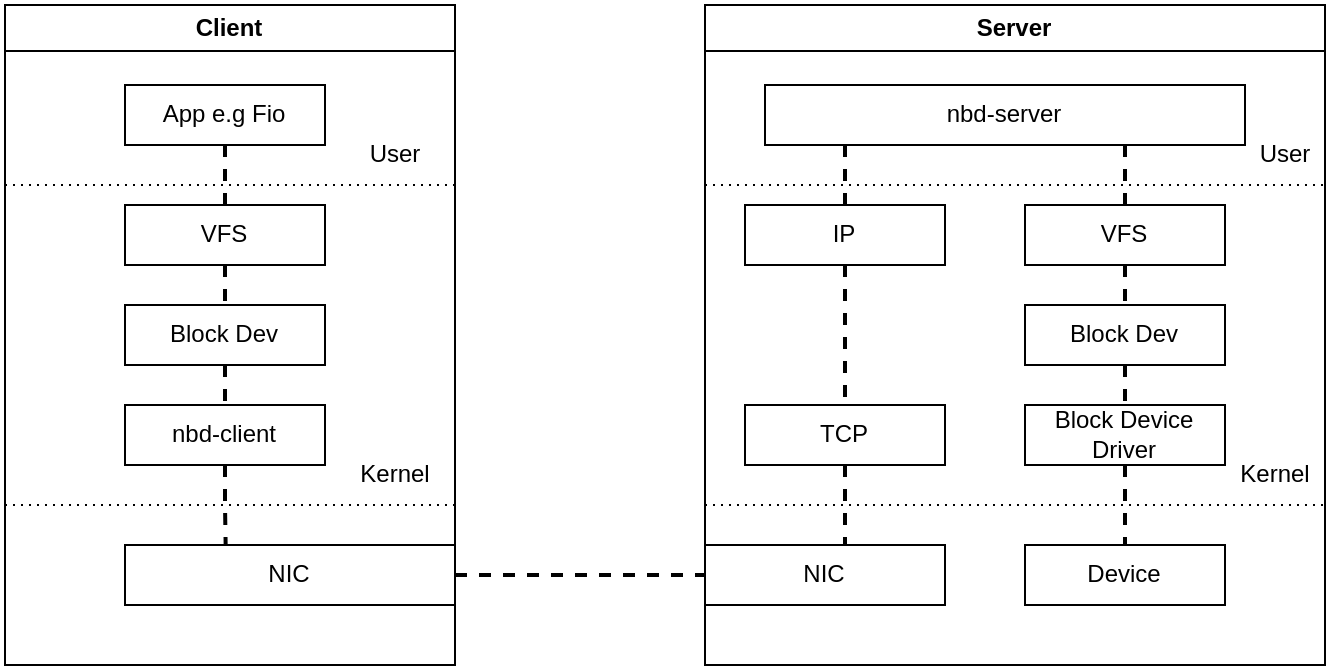
\includegraphics[scale=0.25]{figures/nbd-path2.png}\\
    \caption{I/O Path of NBD system.}
  \end{figure}

\vspace{1em}
\subsection{NvmeOF}
NVMe over Fabrics (NVMe-oF) is a protocol specification designed for connecting
hosts to storage systems over a network using the NVMe protocol. It enables the
transfer of data between a host computer and a target solid-state storage device
or system through network communication. This protocol utilizes NVMe
message-based commands to facilitate data transfers, supporting various
networking technologies such as Ethernet, Fibre Channel (FC), and InfiniBand.

\vspace{1em}
\subsection{SPDK}
The Storage Performance Development Kit (SPDK) is a versatile toolkit tailored
for crafting high-performance, scalable storage applications in user-mode
environments. Its architecture revolves around several core principles aimed at
optimizing performance like User-Space Drivers, Polling Mechanism and lockless
I/O handling. At its foundation, SPDK features a user-space, asynchronous NVMe
driver designed for zero-copy, highly parallel access to SSDs. This driver,
presented as a C library with a simple public header, facilitates seamless
integration for developers. Additionally, SPDK offers a user-space block stack
library mirroring OS functionalities, including storage device interface
unification, queue management for resource constraints, and logical volume
administration. SPDK extends its capabilities with NVMe-oF, iSCSI, and vhost
servers built atop these foundational components.

\note{jk: can you provide more technical context on how SPDK work? This will
help you to explain the figure....}
\note{jk: explain the Figure...}

\begin{figure}[h]
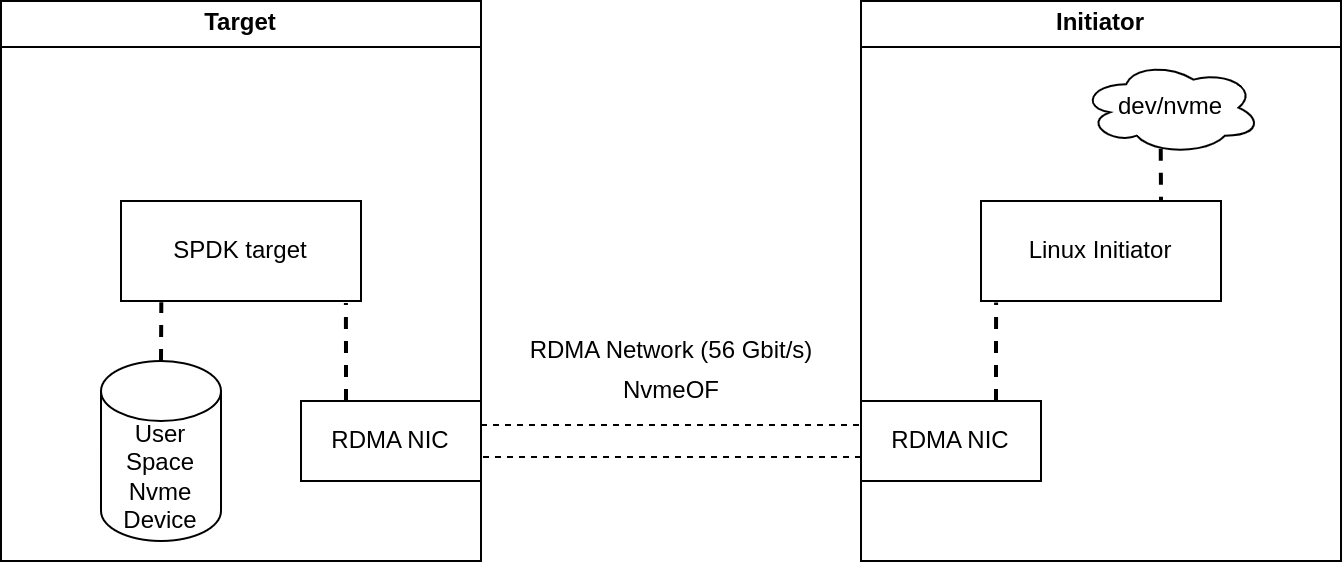
\includegraphics[scale=0.25]{figures/spdk-target.png}\\
\caption{Overview of SPDK NvmeOF Target-Initiator system.}
\end{figure}

\vspace{1em}
\subsection{FIO}
\note{jk: move this to the methodology where we are going to discuss about how
we run the experiments}
Flexible I/O (FIO) Tester, is a widely used open-source tool in the
Linux ecosystem for benchmarking and testing various I/O (input/output)
workloads on storage devices. FIO offers extensive customization options,
enabling users to specify parameters such as block size, I/O pattern
(sequential, random), read/write ratio, queue depth, and concurrency. This
flexibility makes it suitable for evaluating different storage scenarios,
including HDDs, SSDs, NVMe drives, and network storage systems. Additionally,
FIO provides detailed output reports, allowing users to analyze metrics such as
throughput, IOPS (input/output operations per second), latency, and CPU
utilization. We will use FIO for generating I/O 
\vspace{1em}
